\documentclass[a4paper,12pt]{article}
\usepackage{latexsym}
\usepackage{graphicx}
\usepackage{epsfig}
\usepackage{float}
\usepackage{natbib}
\usepackage{listings}
\graphicspath{{./}}
\DeclareGraphicsExtensions{.eps}
\author{Howard Kinsman}
\title{Computational Astrophysics Project 3}
\begin{document}
\maketitle
\section{Problem 1B: Heat Conduction}
\subsection{Part a}
In order to solve this problem it is first necessary to set the initial and boundary conditions. Variables A, B and C were defined according to equation 15 in the notes. Variable A was set to $\mu$ because of $\mu u^n_{j-1}$ in equation 15. In Octave this is simply:
\begin{lstlisting}
A = mu;
\end{lstlisting}
Variable B was set to:
\begin{lstlisting}
B = 1-(2*mu*(1+(1/(j-1))));
\end{lstlisting}
This is in order to satisfy $1-2\mu(1+\frac{1}{j-1})u^n_j$ in equation 15. Finally C was set to:
\begin{lstlisting}
C = mu*(1+(2/(j-1)));
\end{lstlisting}
This satisfies the last part of equation 15: $\mu(1+\frac{2}{j-1})\mu^n_{j+1}$.
\newline
The boundary condition at the surface was set to zero:
\begin{lstlisting}
unew(N) = 0;
\end{lstlisting}
The boundary condition at the centre was set to the value above it on each iteration i.e. the boundary condition at the centre cannot be calculated so it is just assumed to be the same as the value above it. In Octave this was coded as:
\begin{lstlisting}
unew(1) = unew(2);
\end{lstlisting}
The problem required the distributions to be between $\tau=0$ and $\tau=0.2$ so I modified the total time steps to be 2400 because $\Delta_x=1/\left(N-1\right)=\frac{1}{49}$ and so $\Delta_{\tau}=\mu\Delta_x^2=\frac{1}{12005}$ which leads to $n=\frac{\tau_n}{\Delta_{\tau}}+1$ and so $n=2402$.

The plot of the temperature distribution is shown in Fig. \ref{fig:problem1_1}. Each line represents a timestep of 100. At time 1 the temperature gradient is almost vertical as there has been no time for cooling but at a time of 100 the temperature gradient forms a steep curve. The curve gets gradually less steep as time goes on until at time 2400 the curve has flattened considerably and the temperature at the centre has cooled to approximately 0.3.

\begin{figure}[H]
\centering
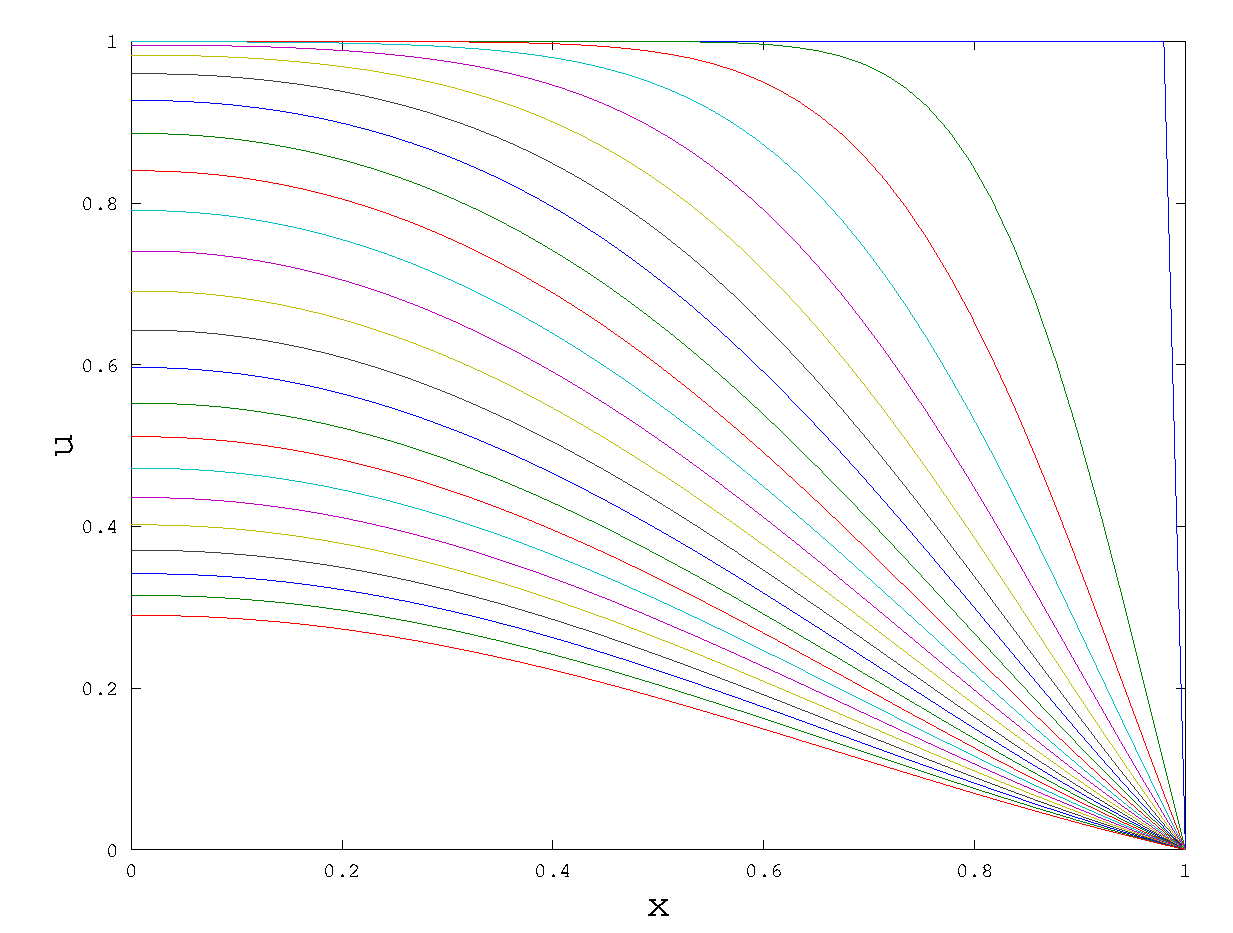
\includegraphics[width=0.75\textwidth]{./problem1_1}
\caption{Plot of temperature distribution}
\label{fig:problem1_1}
\end{figure}

\subsection{Part b}
The following lines of code in Octave retrieve the temperature when it has cooled to exactly half its initial value. The first line retrieves all values at position 2 i.e. the centre (the actual centre is position 1 but this was just set to be the same as position 2 in the boundary conditions). The second line finds the smallest timestep value (n) where temperature (u) is less than 1/2. 
\begin{lstlisting}
u1 = approx(2,:);
nc = min(find(u1<0.5))
\end{lstlisting}
The timestep value n retrieved from the above has a value of 1629. $\tau_n=(n-1)\Delta_{\tau}=\frac{1628}{12005}$. From the notes $\tau$ is in units of $t/\left(a^2/\eta\right)$. Therefore time in seconds=$\tau\left(a^2/\eta\right)$ where $a=100,000m$ and $\eta=10^{-6}m^2 sec$, giving the time it takes the centre to cool to half its initial temperature as $4.3\times 10^7$ years.

Full source code listing for Problem 1B is in Appendix 1.

\newpage
\section{Problem 2: Circular Binary}
\subsection{Part a} 
For a binary system where the centre of mass is at the origin then: $m_1\mathbf{r_1}=m_2\mathbf{r_2}$ and we can express the stars positions using just their mass. The more massive star would lie closer to the centre of mass at a radius that is inversely proportional to its mass.
The equation of motion (for the primary star) is given by:
\begin{equation}
m_p\frac{d^2\mathbf{x_p}}{dt^2}=\frac{Gm_pm_s}{|\mathbf{x_s}-\mathbf{x_p}|^3}\left(\mathbf{x_s}-\mathbf{x_p}\right)
\end{equation}
If we substitute $\mathbf{m_p}=m\mathbf{\tilde{m_p}}$, $\mathbf{x_p}=a\mathbf{\tilde{x_p}}$, $\mathbf{x_s}=a\mathbf{\tilde{x_s}}$ and $t=\tilde{t}\sqrt{a^3/Gm}$ into equation 1 then this leads to:
\begin{equation}
m\mathbf{\tilde{m_p}}\frac{d^2a\mathbf{\tilde{x_p}}}{d\left(\tilde{t}\sqrt{a^3/Gm}\right)^2}=\frac{Gm\mathbf{\tilde{m_p}}m\mathbf{\tilde{m_s}}}{|a\mathbf{\tilde{x_s}}-a\mathbf{\tilde{x_p}}|^3}(a\mathbf{\tilde{x_s}}-a\mathbf{\tilde{x_p}})
\end{equation}
Rearranging, we get:
\begin{equation}
\frac{a\mathbf{\tilde{m_p}}Gm^2d^2\mathbf{\tilde{x_p}}}{a^3d{\tilde{t}}^2}=\frac{Gm^2\mathbf{\tilde{m_p}}\mathbf{\tilde{m_s}}a}{|a\mathbf{\tilde{x_s}}-a\mathbf{\tilde{x_p}}|^3}(\mathbf{\tilde{x_s}}-\mathbf{\tilde{x_p}})
\end{equation}
The $\frac{a\mathbf{\tilde{m_p}}Gm^2}{a^3}$ cancel from both sides leaving:
\begin{equation}
\frac{d^2\mathbf{\tilde{x_p}}}{d\tilde{t}^2}=\frac{\mathbf{\tilde{m_s}}a}{|\mathbf{\tilde{x_s}}-\mathbf{\tilde{x_p}}|^3}(\mathbf{\tilde{x_s}}-\mathbf{\tilde{x_p}})
\end{equation}

The primary star is positioned on the negative side of the x axis, hence $m_scos(\pi)$, whilst the secondary star is on the positive side, hence $m_pcos(0)$. They both sit on the x axis initially so $y=0$. Both of their velocities are zero in the x direction i.e. $-m_ssin(\pi)$ and $-m_psin(0)$ respectively. The stars initial velocities are the time derivatives of the initial positions. The primary star has negative velocity i.e. downwards given by $m_scos(\pi)$ whilst the secondary star has a positive velocity: $m_pcos(0)$, so the orbit is anti-clockwise. 
The initial conditions for this problem are given below. These are assuming an initial phase of $\phi=0$.
\begin{equation}
\mathbf{r_p}=\left(m_scos\left(\pi\right),m_ssin\left(\pi\right)\right)
\end{equation}
\begin{equation}
\mathbf{r_s}=\left(m_pcos\left(0\right),m_psin\left(0\right)\right)
\end{equation}
\begin{equation}
\mathbf{\dot{r_p}}=\left(-m_ssin\left(\pi\right),m_scos\left(\pi\right)\right)
\end{equation}
\begin{equation}
\mathbf{\dot{r_s}}=\left(-m_psin\left(0\right),m_pcos\left(0\right)\right)
\end{equation}

The orbital period is given by:
\begin{equation}
T=2\pi\sqrt{\frac{a^3}{G\left(M_1+M_2\right)}}
\end{equation}
and so in dimensionless units of $\sqrt{\left(a^3/Gm\right)}$ the period is simply $2\pi$.


\subsection{Parts b + c}
Assuming that $\frac{m_p}{m_s}=3$, then $m_p=0.75$ and $m_s=0.25$. I set the final time to be $6\pi$ to allow the stars to orbit three times. In Octave the intial conditions were set as follows:
\begin{lstlisting}
mp    =  .75 ;  % primary mass
ms    =  .25 ;  % secondary mass
x(1)  = ms*cos(pi);  % primary x
x(2)  = ms*sin(pi);  % primary y
x(3)  = -ms*sin(pi);  % primary vx
x(4)  = ms*cos(pi);  % primary vy
x(5)  =  mp*cos(0);  % secondary x
x(6)  =  mp*sin(0);  % secondary y
x(7)  =  -mp*sin(0);  % secondary vx
x(8)  = mp*cos(0);  % secondary vy
tmax  =  6*pi;  % final time
\end{lstlisting}
The full source code listing for Problem 2 is in Appendix 2.

The plot of the two stars is shown in Fig. \ref{fig:problem2_1}. As can be seen the orbits are circular with the more massive primary star (in blue) orbiting closer to the centre of mass. The less massive secondary star (in red) lies much further out. 
\begin{figure}[H]
\centering
\includegraphics[width=0.75\textwidth]{./problem2/problem2_1}
\caption{Plot of circular binary system}
\label{fig:problem2_1}
\end{figure}

\subsection{Part d}
The plot of energy in the system is shown in Fig. \ref{fig:problem2_2}. The plot shows that the derived energy in the system (blue circles) and the exact energy (red line) match. The total energy in the system is constant and negative. The exact energy in the system was calculated using $E_{exact}=\frac{-m_pm_s}{2}$. This is derived as below, for total energy in orbit (potential and kinetic):
\begin{equation}
E=-\frac{Gm_1m_2}{r}+\frac{1}{2}mv^2
\end{equation}
Eliminate v by equating it with gravity:
\begin{equation}
E=-\frac{Gm_1m_2}{r}+\frac{1}{2}G\frac{m_1m_2}{r}
\end{equation}
Kinetic energy therefore is -1/2 of potential energy, so this simplifies to:
\begin{equation}
E=-G\frac{m_1m_2}{2r}
\end{equation}
$E_{exact}=\frac{-m_pm_s}{2}$ is in dimensionless units of $Gm^2/a$.

\begin{figure}[H]
\centering
\includegraphics[width=0.75\textwidth]{./problem2/problem2_2}
\caption{Plot of energy in binary system}
\label{fig:problem2_2}
\end{figure}

\newpage
\section{Problem 3: Hypervelocity Stars}
\subsection{Part a}
In order to plot the stellar orbits in the black hole rest frame it is first necessary to set the initial conditions. As the binary system is moving in a parabola the equations of motion for the centre of mass of parabola are:
\begin{equation}
X_{cm}=(Rcos(f),Rsin(f)),  \qquad  R=\frac{2R_p}{1+cos(f)}     
\end{equation}
This leads to the following equation for the initial angle given that the initial radius is $10R_{tidal}$ and $D=R_p/R_{tidal}=3$:
\begin{equation}
f_0=-cos^{-1}\left(-1+\frac{D}{5}\right)
\end{equation}
because $\frac{2R_p}{10R_{tidal}}=1+cos(f)$.
This was encoded into Octave as:
\begin{lstlisting}
f=-acos(-1+D/5);
\end{lstlisting}
Initial time was set according to the following equation:
\begin{equation}
t_0=\frac{\sqrt{2}}{3}D^{3/2}tan(f_0/2)(3+tan^2(f_0/2))
\end{equation}
In Octave this was set as follows:
\begin{lstlisting}
t = (sqrt(2)/3)*(D^(3/2))*tan(f/2)*(3+(tan(f/2))^2);
\end{lstlisting}
The initial radius is equal to $10R_{tidal}$ and $R_{tidal}=(M/m)^{1/3}a$ so in units of a, R was calculated as follows in Octave:
\begin{lstlisting}
Rt=mb^(1/3);
R=Rt*10;
\end{lstlisting}
The initial positions of the stars relative to the black hole are given by the position of the centre of mass plus the positions of the stars as they orbit each other in circles. The initial position of the centre of mass was calculated as follows:
\begin{lstlisting}
Xx=R*cos(f);
Xy=R*sin(f);
\end{lstlisting}
The initial positions of the stars were calculated in a similar fashion to Problem 2, however a phase of $pi/2$ was used.
In order to calculate the initial velocities of the stars we first need the initial velocity of the centre of mass. This was achieved by taking the derivatives of equation 13 and by using the deriviative of the true anomaly, the angle f:
\begin{equation}
\dot{f}=\frac{\sqrt{2}}{4}D^{-3/2}(1+cos(f))^2
\end{equation}
The above equation is derived from:
\begin{equation}
\frac{df}{dt}=\sqrt{\frac{GM}{R_p^3}}\frac{\sqrt{2}}{4}(1+cos(f))^2
\end{equation}
Here the $\frac{GM}{R_p^3}=D^{-3/2}$ in dimensionless units. We note that $M=R_{tidal}^3$. So therefore it follows that:
\begin{equation}
\sqrt{\frac{GM}{R_p^3}}=\sqrt{\frac{GR_{tidal}^3}{R_p^3}}
\end{equation}
and so, dropping the G for dimensionless units, we have:
\begin{equation}
\sqrt{\frac{R_{tidal}^3}{r_p^3}}=\left(\frac{R_p}{R_{tidal}}\right)^{-3/2}=D^{-3/2}
\end{equation}

The derivative of equation 13 is as follows:
\begin{equation}
\dot{R}=\frac{2R_p\dot{f}sin(f)}{(1+cos(f))^2}
\end{equation}
which gives:
\begin{equation}
\dot{R}=\frac{2R_p\frac{\sqrt{2}}{4}D^{-3/2}sin(f)(1+cos(f))^2}{(1+cos(f))^2}
\end{equation}
This simplies immediately to:
\begin{equation}
\dot{R}=\frac{R_pD^{-3/2}sin(f)}{\sqrt{2}}
\end{equation}
This can be rewritten as:
\begin{equation}
\dot{R}=\frac{R_psin(f)}{D\sqrt{2D}}
\end{equation}
As $D=\frac{R_p}{R_{tidal}}$ and $R_{tidal}=M^{1/3}$ we finally get:
\begin{equation}
\dot{R}=\frac{M^{1/3}sin(f)}{\sqrt{2D}}
\end{equation}

Substituting $\dot{R}$ and $\dot{f}$ into equation 13 and applying the product rule gives us the following equations for $\dot{X_x}$ and $\dot{X_y}$:
\begin{equation}
\dot{X_x}=\dot{R}cos(f)-R\dot{f}sin(f)
\end{equation}
\begin{equation}
\dot{X_y}=R\dot{f}cos(f)+sin(f)\dot{R}
\end{equation}
This was encoded in to Octave as follows:
\begin{lstlisting}
rdot=(mb^(1/3)/(sqrt(2*D)))*sin(f);
fdot=(sqrt(2)/4)*(D^(-3/2))*(1+cos(f))^2;
xdotx=(rdot*cos(f))-(R*fdot*sin(f));
xdoty=(R*fdot*cos(f))+(sin(f)*rdot);
\end{lstlisting}
Finally the initial conditions are ready to be set as follows:
\begin{lstlisting}
x(1) = Xx+(ms*cos(pi/2+pi)); % x : primary star
x(2) = Xy+(ms*sin(pi/2+pi)); % y
x(3) = xdotx+(-ms*sin(pi/2+pi)); % dx/dt
x(4) = xdoty+(ms*cos(pi/2+pi)); % dy/dt
x(5) = Xx+(mp*cos(pi/2)); % x : secondary star
x(6) = Xy+(mp*sin(pi/2)); % y
x(7) = xdotx+(-mp*sin(pi/2)); % dx/dt
x(8) = xdoty+(mp*cos(pi/2)); % dy/dt
\end{lstlisting}

The full source code listing for Problem 3 is in Appendix 3.

Fig. \ref{fig:problem3_1} shows the plot of the stars as the approach the black hole in a parabola. With a penetration factor of $D=\frac{R_p}{R_{tidal}}=3$ they can be seen to be orbitting each other and successfully maintain their orbits as they pass the black hole at periastron.
\begin{figure}[H]
\centering
\includegraphics[width=0.75\textwidth]{./problem3/problem3_1}
\caption{Plot of binary system in BH rest frame where D=3}
\label{fig:problem3_1}
\end{figure}

\subsection{Part b}
Fig. \ref{fig:problem3_2} shows a plot of the same data as in Problem 1 except the plot is in the comoving frame of the secondary star. This was achieved by subtracting the position of the primary star from the position of the secondary star. The was coded into Octave as follows:
\begin{lstlisting}
plot(xs-xp, ys-yp, 'r:')
\end{lstlisting}
\begin{figure}[H]
\centering
\includegraphics[width=0.75\textwidth]{./problem3/problem3_2}
\caption{Plot of primary star in comoving frame of secondary star D=3}
\label{fig:problem3_2}
\end{figure}
The binary system is clearly not destabilised by the black hole.
\subsection{Part c}
Fig. \ref{fig:problem3_3} is a plot of the energy of the binary system. It shows the energy is oscillating from positive to negative between the two stars as they orbit each other. The amplitude of the plot can be seen to be increasing as the stars approach the black hole reaching a maximum at periastron before starting to decrease as they move away from the influence of the black hole. The system has a total energy of zero and the energy of the one star is always the negative of the other.
\begin{figure}[H]
\centering
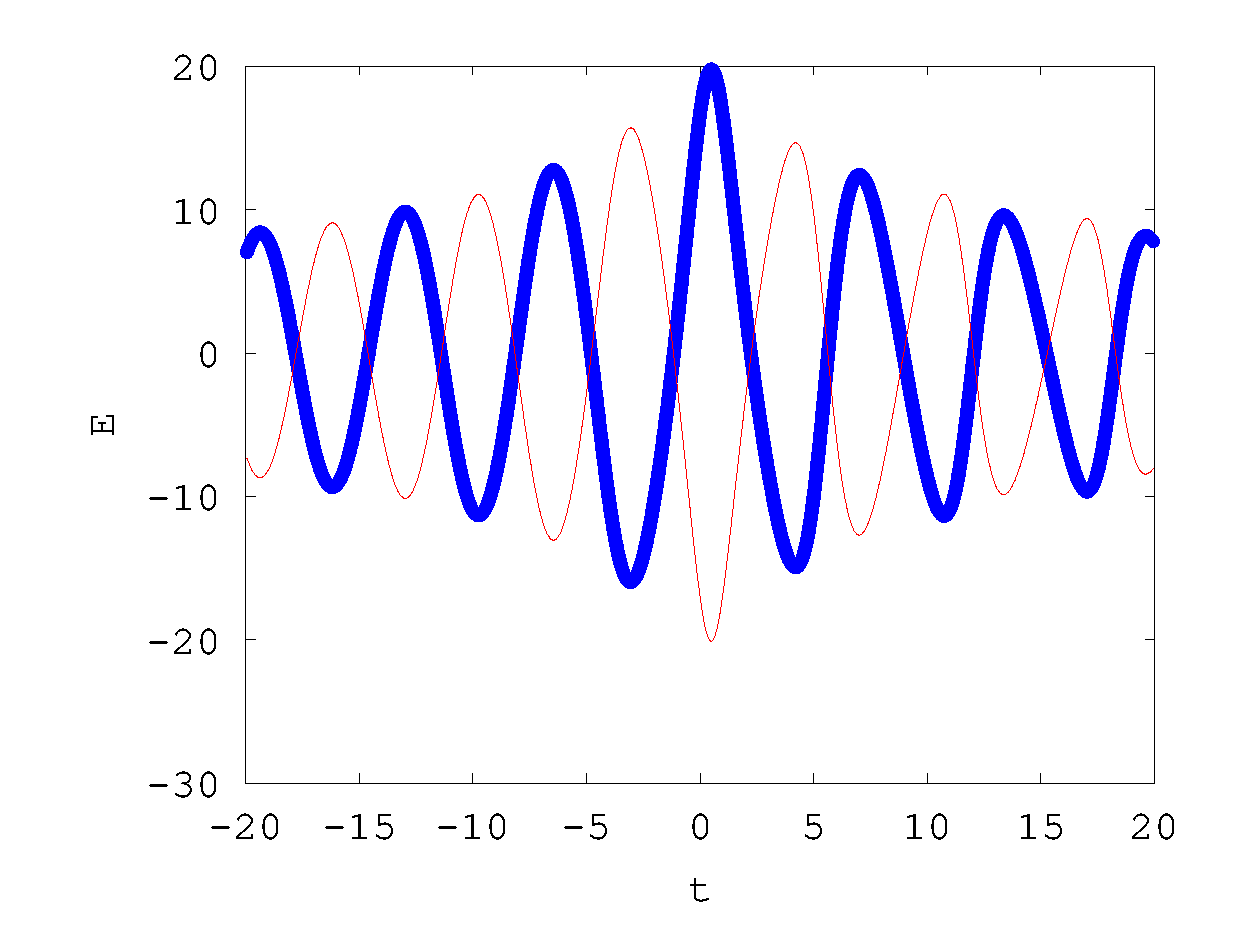
\includegraphics[width=0.75\textwidth]{./problem3/problem3_3}
\caption{Plot of energy in binary system D=3}
\label{fig:problem3_3}
\end{figure}

\subsection{Part d}
The code was then re-run but this time with $R_p=0.1R_{tidal}$.
Fig. \ref{fig:problem3_4} is a plot again in the rest frame of the black hole.
The binary system is clearly disrupted by the black hole. The two stars are orbitting each until the closest approach to the black hole where they separate.
\begin{figure}[H]
\centering
\includegraphics[width=0.75\textwidth]{./problem3/problem3_4}
\caption{Plot of binary system in BH rest frame where D=0.1}
\label{fig:problem3_4}
\end{figure}

A plot of the secondary star in the comoving frame of the primary star, Fig. \ref{fig:problem3_5}, shows the secondary star to be initially in orbit with the primary star but then leaves the binary system on a separate trajectory.
\begin{figure}[H]
\centering
\includegraphics[width=0.75\textwidth]{./problem3/problem3_5}
\caption{Plot of primary star in comoving frame of secondary star D=0.1}
\label{fig:problem3_5}
\end{figure}

A plot of the energy of the system, Fig. \ref{fig:problem3_6}, shows that the energy is initially oscillating as in Part c but after the closest approach to the black hole the energy no longer oscillates between the two stars after the system is disrupted. The primary star (blue) ends up with a high negative energy whilst the secondary star (red) has a high positive energy.
\begin{figure}[H]
\centering
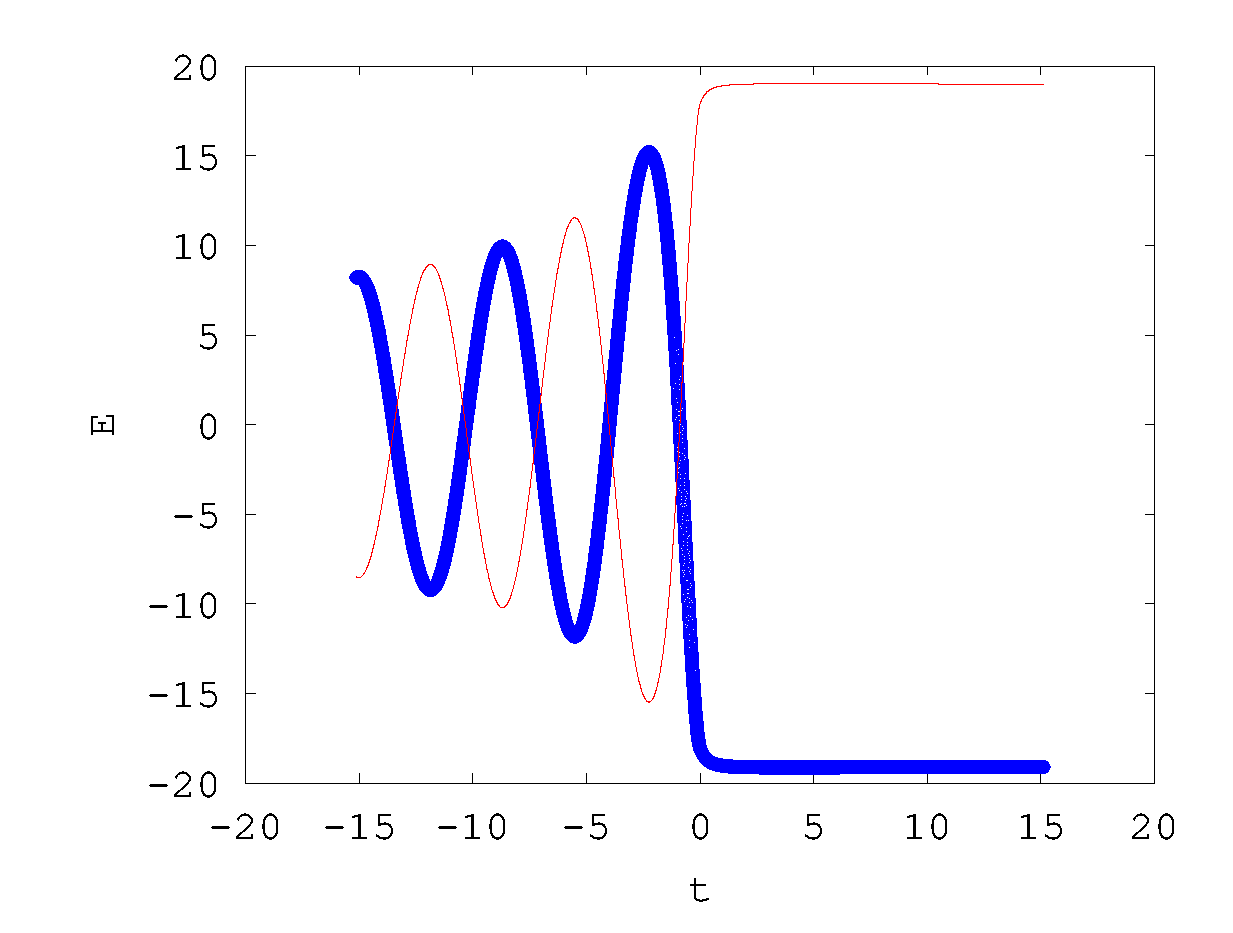
\includegraphics[width=0.75\textwidth]{./problem3/problem3_6}
\caption{Plot of energy in binary system D=0.1}
\label{fig:problem3_6}
\end{figure}

\subsection{Part e}
The velocity of the ejected star (secondary star in this case) can be calculated by using $E_k=1/2mv^2$ so
\begin{equation}
v=\sqrt{2E/M}
\end{equation}
From Fig. \ref{fig:problem3_6}, and from the output file, the energy of the ejected star tends towards 19 as r approaches $\infty$. E here is in units of $Gm^2/a$ so, in kms units, $Gm^2/a=5.4\times10^{40}$ and so $E=10^{41}J$. From equation 27 we get 1,017,849m/s, and so the ejected star is travelling at approximately 1000km/s at $r=\infty$.
\subsection{Part f}
Throughout this project I had assumed that the lower mass star would always be ejected from the system, so I chose to investigate this further to see if my assumptions were correct.
I ran the above simulation 8 times whilst varying the initial phase of the binary system i.e. pi/4, pi/2, 3pi/4, pi, 5pi/4, 3pi/2, 7pi/4 and 2pi.
The results were surprsing because in exactly half the runs the lower mass star was ejected and half the larger mass star. With an initial phase of pi/4 to pi the lower mass star was ejected, whilst from 5pi/4 to 2pi the larger mass star was ejected, see Fig. \ref{fig:problem3_7}. This suggests that this process is independent of the mass of the star.
\begin{figure}[H]
\centering
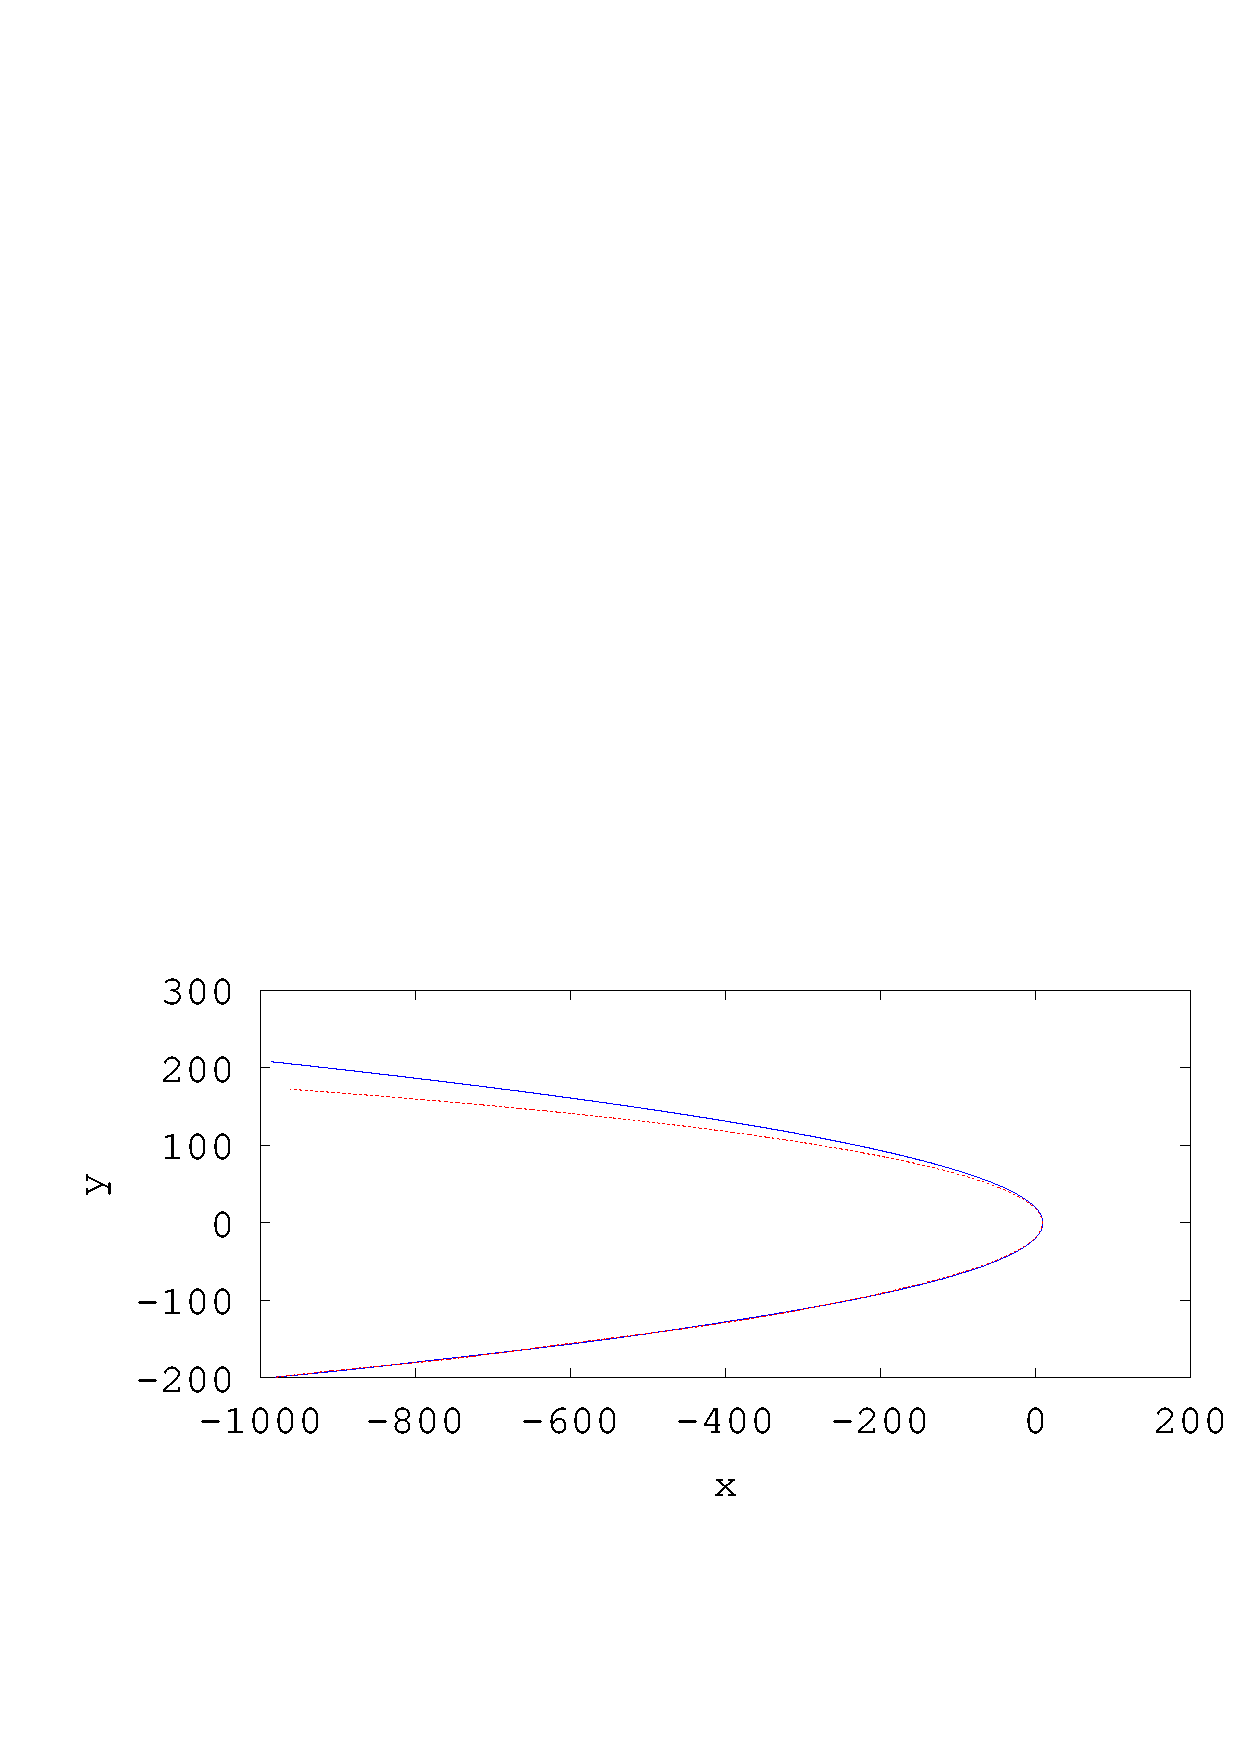
\includegraphics[width=0.75\textwidth]{./problem3/problem3_7}
\caption{Plot of binary system in BH rest frame where D=0.1 and Phase=2Pi}
\label{fig:problem3_7}
\end{figure}
This may be possibly due to the energy in the system. The total energy in the system is zero so the energy of the one star is always equal to the negative of the other. The star which is ejected may be the one that is in the phase with positive energy at the time of closest approach to the black hole. 

Astronomical observations could confirm whether indeed we do detect similar numbers of high mass hypervelocity stars as we do low mass hypervelocity stars.
\newpage
\section{Appendix 1 - Problem 1B code}
\lstinputlisting[language=Octave]{Part2.m}
\newpage
\section{Appendix 2 - Problem 2 code}
\lstinputlisting[language=Octave]{./problem2/binary.m}
\lstinputlisting[language=Octave]{./problem2/f.m}
\lstinputlisting[language=Octave]{./problem2/energy.m}
\lstinputlisting[language=Octave]{./problem2/RK4.m}
\lstinputlisting[language=Octave]{./problem2/orbitplot.m}
\lstinputlisting[language=Octave]{./problem2/energyplot.m}
\newpage
\section{Appendix 3 - Problem 3 code}
\lstinputlisting[language=Octave]{./problem3/initialc.m}
\lstinputlisting[language=Octave]{./problem3/f.m}
\lstinputlisting[language=Octave]{./problem3/HVS.m}
\lstinputlisting[language=Octave]{./problem3/script4.m}
\lstinputlisting[language=Octave]{./problem3/RK4.m}
\lstinputlisting[language=Octave]{./problem3/energy.m}
\end{document}


